\documentclass{article}
%%
%% Author: maciejsrokowski
%% 11/07/2018
%%

% Packages
\usepackage{a4wide}
\usepackage{amsmath}
\usepackage{physics}
\usepackage{siunitx}
\usepackage{graphicx}
\usepackage{cancel}

% Document
\begin{document}

    \title{Vectors}
    \maketitle
    \newtheorem{theorem}{Theorem}
    \newtheorem{definition}{Definition}
    \newtheorem{example}{Example}
    \newtheorem{problem}{Problem}

    \section{Vectors}

    Every vector has a:
    \begin{itemize}
        \item Magnitude - that is just length and is obtainable by using pythagorean theorem on all components
        \item Unit vector - (Denoted as $\vu{u}$)that is a vector with the same direction as the original vector but of the magnitude 1. To obtain it you have to divide every component by the magnitude of the original vector
    \end{itemize}

    \section{Dot product}

    A way of multiplying two vectors to get a \textbf{scalar}
    \[\va{A}\cdot\va{B}=\sum{a_ib_i}=\cancel{a_1b_1}+a_2b_2+a_3b_3+\dots\]
    What is it good for? It gives us info about lengths and angles because (this can also be quite a good proof for lat of cosines) It is called dot product because the symbol used for it is a dot! Because the result is a scalar it is also called scalar product:
    \[\va{A}\cdot\va{B}=\abs*{\va{A}}\abs*{\va{B}}\cos{\theta}\]



    \begin{problem}
        \begin{itemize}
            \item[a)]Compute $\bmqty{1 & 2 & -4}\cdot\bmqty{2 & 3 & 5}$
            \[
                \bmqty{1 & 2 & -4}\cdot\bmqty{2 & 3 & 5}=2+6-20=-12
            \]
            \item[b)] Is the angle between these two vectors acute, obtuse or right?\\
            The dot product is negative so $\cos{\theta}<$ and that means that $\theta > \frac{\pi}{2}$. The angle is obtuse
        \end{itemize}
    \end{problem}

    \begin{problem}
        Suppose $B=\bmqty{2 & 2 & 1}$. Suppose also that B makes an angle of $\ang{30}$ with A and $A\cdot B=6$. Find $\abs{A}.$\\
        \begin{align}
            \sqrt{4 + 4 +1}\cdot\abs{A}\cos{\ang{30}}=6\\
            \abs{A}=\frac{6\cdot2}{3\cdot\sqrt{3}}=\frac{4}{\sqrt{3}}
        \end{align}
    \end{problem}

    \begin{problem}
        If $A\cdotB=0$ what is the angle between A and B?\\
        The angle is right or magnitudes of one or both vectors are zero
    \end{problem}

    \begin{problem}
        Using vectors and dot product show the diagonals of a parallelogram have equal lengths if and only if it's a rectangle
        \paragraph{Answer}
        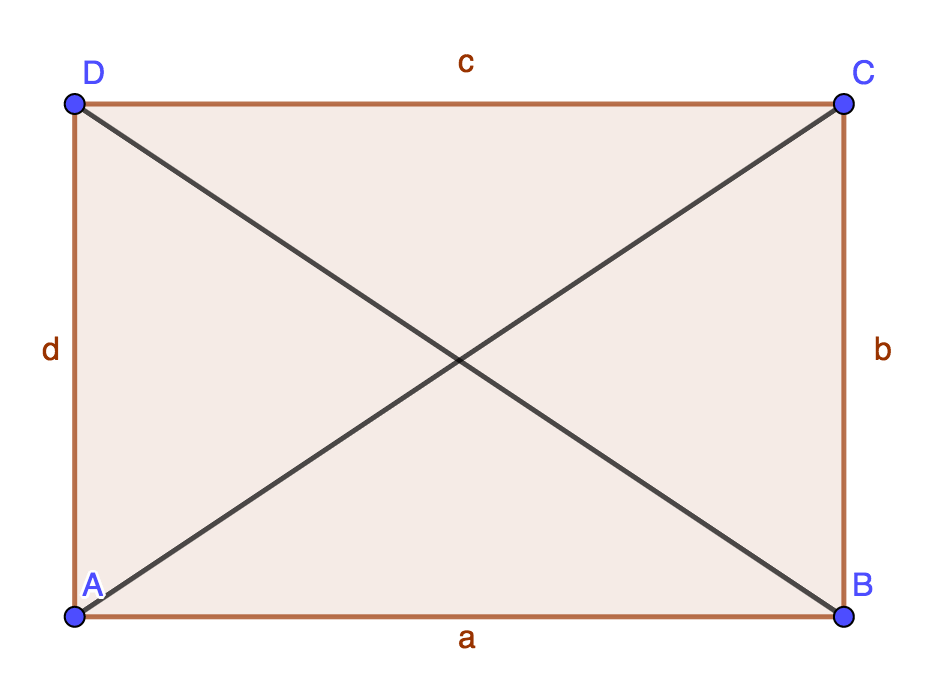
\includegraphics[width=0.25\textwidth]{fig_1.png}
        We require that
        \[\abs{\va{AC}}=\abs{\va{DB}}\]
        We can show this by using the fact that:
        \[\va{v}\vdot\va{v}=\abs{v}^2\]
        So that
        \begin{gather}
            \va{AC}=\va{AB}+\va{BC}\\
            \va{DB}=\va{DA}+\va{AB}=\va{AB}-\va{BC}\\
            \abs{AC}^2=(\va{AB}+\va{BC})\vdot(\va{AB}+\va{BC})
            =\abs{\va{AB}}^2+2\va{AB}\vdot\va{BC}+\abs{\va{BC}}^{2}\\
            \abs{DB}^2=(\va{AB}-\va{BC})\vdot(\va{AB}-\va{BC})
            =\abs{\va{AB}}^2-2\va{AB}\vdot\va{BC}+\abs{\va{BC}}^2
        \end{gather}

        From the above we imply that:
        \begin{gather}
            \abs{\va{AC}}=\abs{\va{DB}\leftrightarrow}
            \abs{\va{AB}}^2+2\va{AB}\vdot\va{BC}+\abs{\va{BC}}^{2}=
            \abs{\va{AB}}^2-2\va{AB}\vdot\va{BC}+\abs{\va{BC}}^{2}\\
            \abs{\va{AC}}=\abs{\va{DB}}\leftrightarrow
            4\va{AB}\vdot\va{BC}=0
        \end{gather}
        That means that $\abs{\va{AC}}=\abs{\va{DB}}$ only when $\va{AB}$ and $\va{BC}$ are orthogonal (their dot product equals 0). QED

    \end{problem}

    \begin{problem}
        Find the andle between the vectors $A=i+8j$ and $B=i+2j$
        \paragraph{Answer}
        \[
            \cos{\theta}=\frac{1 + 16}{\sqrt{1+8^2}\cdot\sqrt{1+2^2}}=\frac{17}{\sqrt{65}\sqrt{5}}
        \]
    \end{problem}

    \begin{problem}
        Take points $P=(a, 1, -1), Q=(0,1,1),R=(a,-1,3)$. For what value(s) of a is PQR a right angle?
        \paragraph{Answer}
        \begin{gather}
            \va{QP}=P-Q=\bmqty{a & 0 & -2}\\
            \va{QR}=R-Q=\bmqty{a & -2 & 2}\\
            \va{QP}\vdot\va{QR}=a^2 + 0 - 4 = 0\\
            a=\pm2
        \end{gather}
    \end{problem}

    \begin{problem}
        Show that the diagonals of a parallelogram are perpendicular if and only id it is a rhombus, i.e., it's four sides have equal lengths
        \paragraph{Answer}
        The diagonals are perpendicular only if
        \begin{gather}
            \va{AC}\vdot\va{DB}=0\\
        \end{gather}
        The diagonals can be described as
        \begin{gather}
            \va{AC}=\va{AB} + \va{BC}\\
            \va{DB}=\va{DA} + \va{AB} = \va{AB} - \va{BC}\\
        \end{gather}
        Substituting:
        \begin{gather}
            (\va{AB} + \va{BC})\vdot(\va{AB} - \va{BC})=0\\
            \va{AB}^2 + \va{BC}^2 = 0\\
            \abs{\va{AB}}^2 + \abs{\va{BC}}^2 = 0
        \end{gather}
        Since $\va{AB} = \va{CD}$ and $\va{BC} = \va{DA}$ all the edges have to be equal
        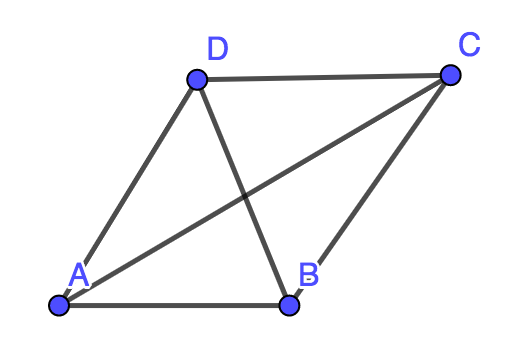
\includegraphics[width=0.25\textwidth]{fig_2.png}


    \end{problem}


    \subsection{Angle - sign}

    The sign of dot product will be:
    \begin{align}
        \va{A}\cdot\va{B}>0\qq{if}\theta<\ang{90}\\
        \va{A}\cdot\va{B}<0\qq{if}\theta>\ang{90}\\
        \va{A}\cdot\va{B}=0\qq{if}\theta=\ang{90}\\
    \end{align}


    \subsection{Definition of a plane by vectors}

    Equation in the form of $3x+4y+z=0$ describes a plane because if we take dot product of a vector $\va{A}=\bmqty{3&4&1}$ and any vector $\va{P}$. Then $\va{A}\vdot\va{P}=0$. That implies any vector $\va{P}$ is perpendicular do vector $\va{A}$

    \section{Vector components}

    Components of $\va{A}$ along the $\vu{u}$ (unit vector).

    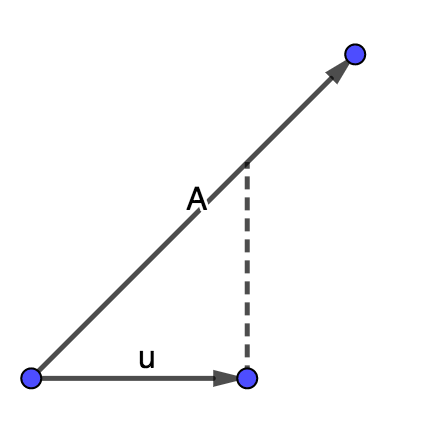
\includegraphics[width=0.25\textwidth]{fig_3.png}

    \[component=\va{A}\vdot\vu{u}=\abs{\va{A}}\abs{\vu{u}}\cos{\theta}=\abs{\va{A}}\cos{\theta}\]

    The remainder of the vector $\va{A}$ that is parallel to $\vu{u}$ is also called \emph{orthogonal projection} of $\va{A}$ on unit vector $\vu{u}$

    \begin{problem}
        Find the component of \textbf{A} in the direction of \textbf{B}
        \begin{itemize}
            \item i) $\abs{\va{A}}=2, \abs{\va{B}}=5, \theta=\frac{\pi}{4}$\\r
            \[component=\abs{\va{A}}\cos{\theta}=2\cdot\frac{\sqrt{2}}{2}=\sqrt{2}\]
            \item ii) $\va{A}=i + 2j, \va{B}=3i+4j$
            \[\vu{u}\text{ (in direction B) }=\frac{B}{\abs{\va{B}}}=\frac{3}{5}i+\frac{4}{5}j\]
            \[component=\vu{u}\cdot\va{A}=\frac{3}{5}+\frac{4}{5}\cdot2=\frac{11}{5}\]
        \end{itemize}
    \end{problem}

    \section{Area}

    How to calculate the area using vectors?

    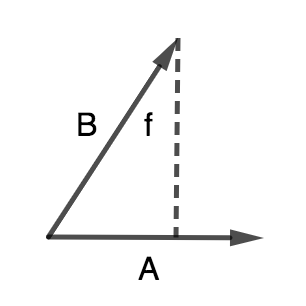
\includegraphics[width=0.35\textwidth]{fig_4.png}

    We can calculate area in the following way
    \[Area=\frac{1}{2}\abs{\va{A}}\abs{\va{B}}\sin{\theta}\]
    Unfortunately this contains sin instead of cos. It's time to introduce $A^\prime$.  $A^\prime$ is A rotated $\ang{90}$. Thus:
    \[\cos{\theta^\prime}=\sin{\theta}\]
    \begin{align}
        & \abs{\va{A}}\abs{\va{B}}\sin{\theta}\\
        & =\abs{\va{A^\prime}}\abs{\va{B}}\cos{\theta^\prime}\\
        & =\va{A^\prime}\vdot\va{B}
    \end{align}

    How to find $\va{A^\prime}$?

    \[\va{A^\prime}=\bmqty{-a_2 & a_1}\]

    Let's calculate further:

    \begin{align}
        & \va{A^\prime}\vdot\va{B}\\
        & =\bmqty{-a_2 & a_1}\vdot\bmqty{b_1 & b_2}\\
        & =a_1 b_2 - a_2 b_1 \\
        & =det(\va{A}, \va{B})
    \end{align}

    It is a determinant, the determinant measures the area of the whole parallelogram:

    \[\det(\va{A}, \va{B})= \mdet{a_1 & a_2 \\ b_1 & b_2}=a_1 b_2 - a_2 b_1\]

    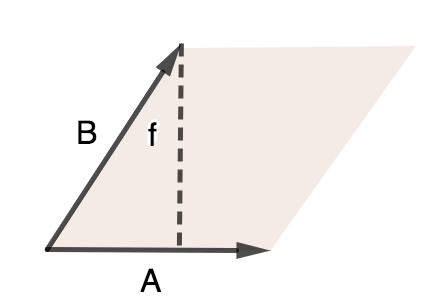
\includegraphics[width=0.35\textwidth]{fig_5.png}

    \section{Volues and Determinants in space}

    We have 3 vectors $\va{A}$, $\va{B}$ and $\va{C}$. Their determinant will be:

    \begin{align}
        \det(\va{A}, \va{B}, \va{C})
        =\mdet{
        a_1 & a_2 & a_3 \\
        b_1 & b_2 & b_3 \\
        c_1 & c_2 & c_ 3
        }
        =a_1 \mdet{b_2 & b_3 \\ c_2 & c_3 }
        -a_2 \mdet{b_1 & b_3 \\ c_1 & c_3}
        +a_3 \mdet{b_1 & b_2 \\ c_1 & c_2}
    \end{align}

    \begin{theorem}
        \[\det(\va{A}, \va{B}, \va{C})=\pm\text{\emph{volume of a parallelepiped}}\]
    \end{theorem}

    Important facts about $\det(A)$ :
    \begin{itemize}
        \item D-1. $\det(A)$ is multiplied by $−1$ if we interchange two rows or two columns.
        \item D-2. $\det(A)$ = 0 if one row or column is all zero, or if two rows or two columns are the
        same.
        \item D-3. $\det(A)$ is multiplied by c, if every element of some row or column is multiplied by c.
        \item D-4. The value of $\det(A)$ is unchanged if we add to one row (or column) a constant multiple
        of another row (resp. column).
    \end{itemize}

    \subsection{Entries, minors and cofactors}

    \begin{itemize}
        \item Matrix entry, written as $a_{ij}$ is and element of the matrix at i-th row and j-th column
        \item Matrix minor ,written as $\abs{A_{ij}}$ or $\det(A_{ij})$, is the determinant that's left after deleting from $\abs{A}$ the row and column containing $a_{ij}$
        \item Matrix determinant ij-cofactor, written as $A_{ij}$, is given as a formula by $A_{ij} = (-1)^{i+j}\abs{A_{ij}}$. For a $3 \cross 3$ determinant, it is easier to think of it this way: we put + or − in front of the ij-minor, according to whether + or − occurs in the ij-position in the checkerboard pattern
        \[
            \mdet{
            + & - & +\\
            - & + & -\\
            + & - & +
            }
        \]
        \begin{example}
            \[
                \mdet{
                1 & 0 & 3\\
                1 & 2 & -1\\
                2 & 1 & -1
                }
            \]
            Find $\abs{A_{12}}, A_{12}, \abs{A_{22}}, A_{22}$
            \[
                \abs{A_{12}} = \mdet{1 & -1\\ 2 & -1} =1, A_{12} = -1\\
                \abs{A_{22}} = \mdet{1 & 3\\ 2 & -1} =1, A_{22} = -7\\

            \]
        \end{example}
    \end{itemize}

    \section{Laplace expansion by cofactors}

    This is another way to evaluate a determinant; we give the rule for a $3 \cross 3$. It generalizes easily to an $n \cross n$ determinant.
    Select any row (or column) of the determinant. Multiply each entry aij in that row (or column) by its cofactor Aij, and add the three resulting numbers; you get the value of the determinant.

    As practice with notation, here is the formula for the Laplace expansion of a third order (i.e., a $3 \cross 3$) determinant using the cofactors of the first row:


    \[ a_{11}A_{11} + a_{12}A_{12} + a_{13}A_{13} = \abs{A} \]

    As you can see this is just a generalization of the method from previous section. The cofactors are what gives - sign in second term of the resolution in previous sections

    \section{Cross product}

    Cross product (also called vector product) is a product of 2 vectors in 3D space. The result is also a vector

    \begin{definition}
        \begin{align}
            \va{A}\cross\va{B}
            =\mdet{
            \vu{i} & \vu{j} & \vu{k}\\
            a_1 & a_2 & a_3 \\
            b_1 & b_2 & b_3
            }
            =\vu{i}\mdet{a_2 & a_3 \\ b_2 & b_3}
            -\vu{j}\mdet{a_1 & a_3 \\ b_1 & b_3}
            +\vu{k}\mdet{a_1 & a_2 \\ b_1 & b_2}
        \end{align}
    \end{definition}

    \begin{theorem}
        Geometrically
        \begin{itemize}
            \item $\abs{\va{A} \cross \va{B}}=\text{area of parallelogram}$
            \item Direction $\va{A} \cross \va{B}$ is $\perp$ to the plane on which $\va{A}$ and $\va{B}$ are on
        \end{itemize}
    \end{theorem}

    \begin{theorem}
        The magnitude of the cross product:
        \begin{align}
            \abs{\va{A} \cross \va{B}} = \abs{\va{A}}\abs{\va{B}}\sin{\theta}
        \end{align}
    \end{theorem}

    \subsection{The right-hand rule}

    In doing cross production of $\va{A} \cross \va{B}$
    \begin{itemize}
        \item Pointing finger points in the direction of $\va{A}$
        \item Middle finger points in the direction of $\va{B}$
        \item Thumb points in the direction $\va{A} \cross \va{B}$
    \end{itemize}

    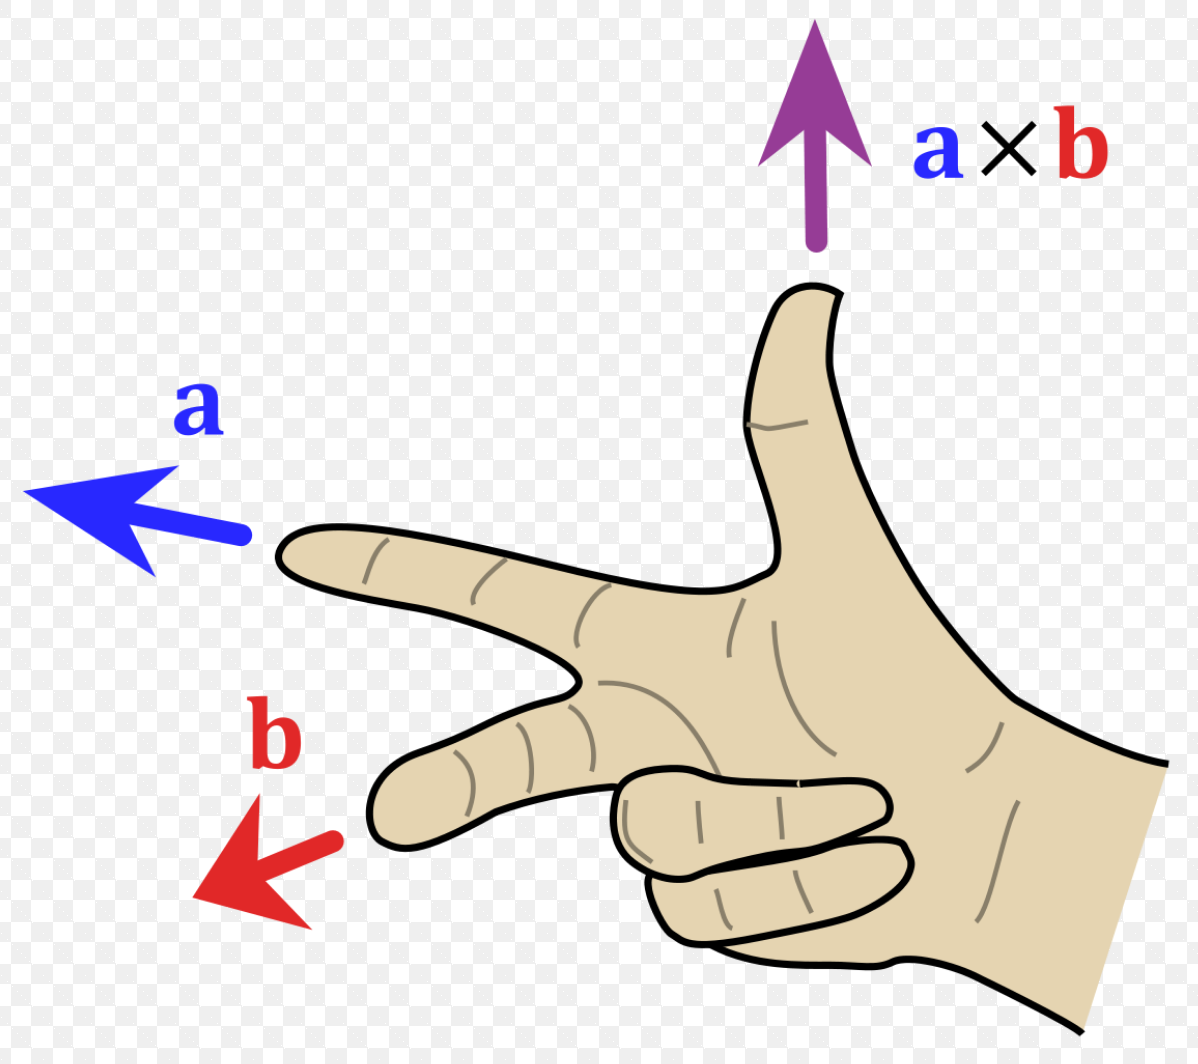
\includegraphics[width=0.25\textwidth]{fig_6.png}

    \subsection{Obtaining volume by cross product, triple product}

    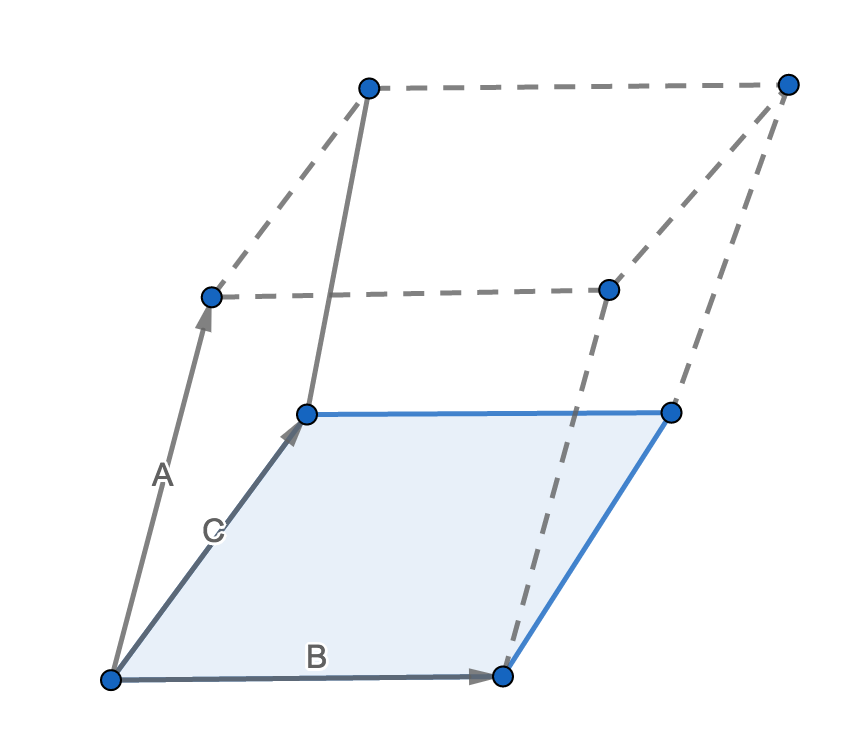
\includegraphics[width=0.25\textwidth]{fig_7.png}

    Volume of parallelepiped equals the area of the base times the height (h):

    \begin{align}
        V & =\abs{\va{B} \cross \va{C}}(\va{A}\vdot\vu{h})\\
        & =\cancel{\abs{\va{B} \cross \va{C}}}
        (\va{A}\vdot\frac{\va{B} \cross \va{C}}{\cancel{\abs{\va{B} \cross \va{C}}}})\\
        & =\va{A}\vdot(\va{B} \cross \va{C})
    \end{align}

    The result of this equation is called \textbf{triple product} and

    \begin{align}
        \det(\va{A}, \va{B}, \va{C})=\va{A}\vdot(\va{B} \cross \va{C})
    \end{align}

    \subsection{Cross product properties}

    Cross product is not commutative

    \begin{align}
        \va{A} \cross \va{B} \cancel{=} \va{B} \cross \va{A}
    \end{align}

    Althought the cross product length stays the same in both cases

    \begin{align}
        \abs{\va{A} \cross \va{B}} =  \abs{\va{B} \cross \va{A}}
    \end{align}

    The direction is of the product is reversed so it is \textbf{anti-commutative}

    \begin{align}
        \va{A} \cross \va{B} = - \va{B} \cross \va{A}
    \end{align}

    Cross product is \textbf{distributive}:

    \begin{align}
        \va{A} \cross (\va{B} + \va{C}) = \va{A} \cross \va{B} + \va{A}\cross \va{C}
    \end{align}

    Cross product is \textbf{non-associative}

    \begin{align}
        (\va{A} \cross \va{B} ) \cross \va{C} \cancel{=} \va{A} \cross (\va{B} \cross \va{B})
    \end{align}

    \begin{problem}
        Compute $(i + 2j) \cross (2i - 3j)$

        \begin{align}
            (i + 2j) \cross (2i - 3j)
            =\bmqty{
            i & j & k \\
            1 & 2 & 0\\
            2 & -3 & 0
            }
            =0i + 0j -7k
            = -7k
        \end{align}
    \end{problem}

    \subsection{Equation of a plane}

    Given points $P_1 , P_2 , P_3$ describing a plane find if point $P$ lays is the same plane\\
    They are if $\det((\va{PP_1}), (\va{PP_2}), (\va{PP_3}))=0$\\\\
    We can also do this using cross product:\\
    P is on a plane $\leftrightarrow \va{PP_1} \perp \va{N}$ where N is some vector perpendicular to the plane\\
    P is on a plane $\leftrightarrow \va{PP_1} \vdot \va{N}=0$\\
    How to find N?\\
    $\va{N}=\va{P_1 P_2} \cross \va{P_1 P_3}$\\
    Substituting, we again get triple product:
    P is on a plane $\leftrightarrow \va{PP_1} \vdot (\va{P_1 P_2} \cross \va{P_1 P_3})=0$\\


\end{document}